% Digital Logic Report Template
% Created: 2020-01-10, John Miller

%==========================================================
%=========== Document Setup  ==============================

% Formatting defined by class file
\documentclass[11pt]{article}

% ---- Document formatting ----
\usepackage[margin=1in]{geometry}	% Narrower margins
\usepackage{booktabs}				% Nice formatting of tables
\usepackage{graphicx}				% Ability to include graphics

%\setlength\parindent{0pt}	% Do not indent first line of paragraphs 
\usepackage[parfill]{parskip}		% Line space b/w paragraphs
%	parfill option prevents last line of pgrph from being fully justified

% Parskip package adds too much space around titles, fix with this
\RequirePackage{titlesec}
\titlespacing\section{0pt}{8pt plus 4pt minus 2pt}{3pt plus 2pt minus 2pt}
\titlespacing\subsection{0pt}{4pt plus 4pt minus 2pt}{-2pt plus 2pt minus 2pt}
\titlespacing\subsubsection{0pt}{2pt plus 4pt minus 2pt}{-6pt plus 2pt minus 2pt}

% ---- Hyperlinks ----
\usepackage[colorlinks=true,urlcolor=blue]{hyperref}	% For URL's. Automatically links internal references.

% ---- Code listings ----
\usepackage{listings} 					% Nice code layout and inclusion
\usepackage[usenames,dvipsnames]{xcolor}	% Colors (needs to be defined before using colors)

% Define custom colors for listings
\definecolor{listinggray}{gray}{0.98}		% Listings background color
\definecolor{rulegray}{gray}{0.7}			% Listings rule/frame color

% Style for Verilog
\lstdefinestyle{Verilog}{
	language=Verilog,					% Verilog
	backgroundcolor=\color{listinggray},	% light gray background
	rulecolor=\color{blue}, 			% blue frame lines
	frame=tb,							% lines above & below
	linewidth=\columnwidth, 			% set line width
	basicstyle=\small\ttfamily,	% basic font style that is used for the code	
	breaklines=true, 					% allow breaking across columns/pages
	tabsize=3,							% set tab size
	commentstyle=\color{gray},	% comments in italic 
	stringstyle=\upshape,				% strings are printed in normal font
	showspaces=false,					% don't underscore spaces
}

% How to use: \Verilog[listing_options]{file}
\newcommand{\Verilog}[2][]{%
	\lstinputlisting[style=Verilog,#1]{#2}
}




%======================================================
%=========== Body  ====================================
\begin{document}

\title {ELC 2137 Lab 01: Git and LaTeX Intro}
\author {Justin Woods}

\maketitle


\section*{Summary}

The purpose of the lab was to learn how to set up and operate the version control software GitHub and the typesetting language LaTeX.
 GitHub is helpful because it keeps track of file modifications and allows for easy collaboration with others.
  LaTeX is helpful for producing professional-looking documents. 


\section*{Q\&A}

\begin{enumerate}
	
	\item What is your GitHub user name?
	
	JustinWoods1
	
	\item What LaTeX environment produces a bulleted list?

	
	 itemize
	 
	\item Write the equation \verb|y(t) = 1/2 e\^t| using LaTeX equation formatting.
	
		 $y(t) = 1/2 e^t$
	 
	\item What is the shortcut key for compiling your LaTeX document?
	
	F5
	
	
\end{enumerate}

\section*{Code}

\Verilog{example_or.sv}

\section*{Results}

\begin{figure}[ht]\centering 
	
	\begin{tabular}{c|c|c}
		\toprule
		Binary & Hex & Decimal \\
		\midrule
		0000   & 0 & 0 \\
		0010   & 2 & 0 \\
		1100   & 4 & 0 \\
		0110   & 6 & 6 \\ 
		1000   & 8 & 8 \\
		1010   & A & 10 \\
		\bottomrule	
	\end{tabular}  

		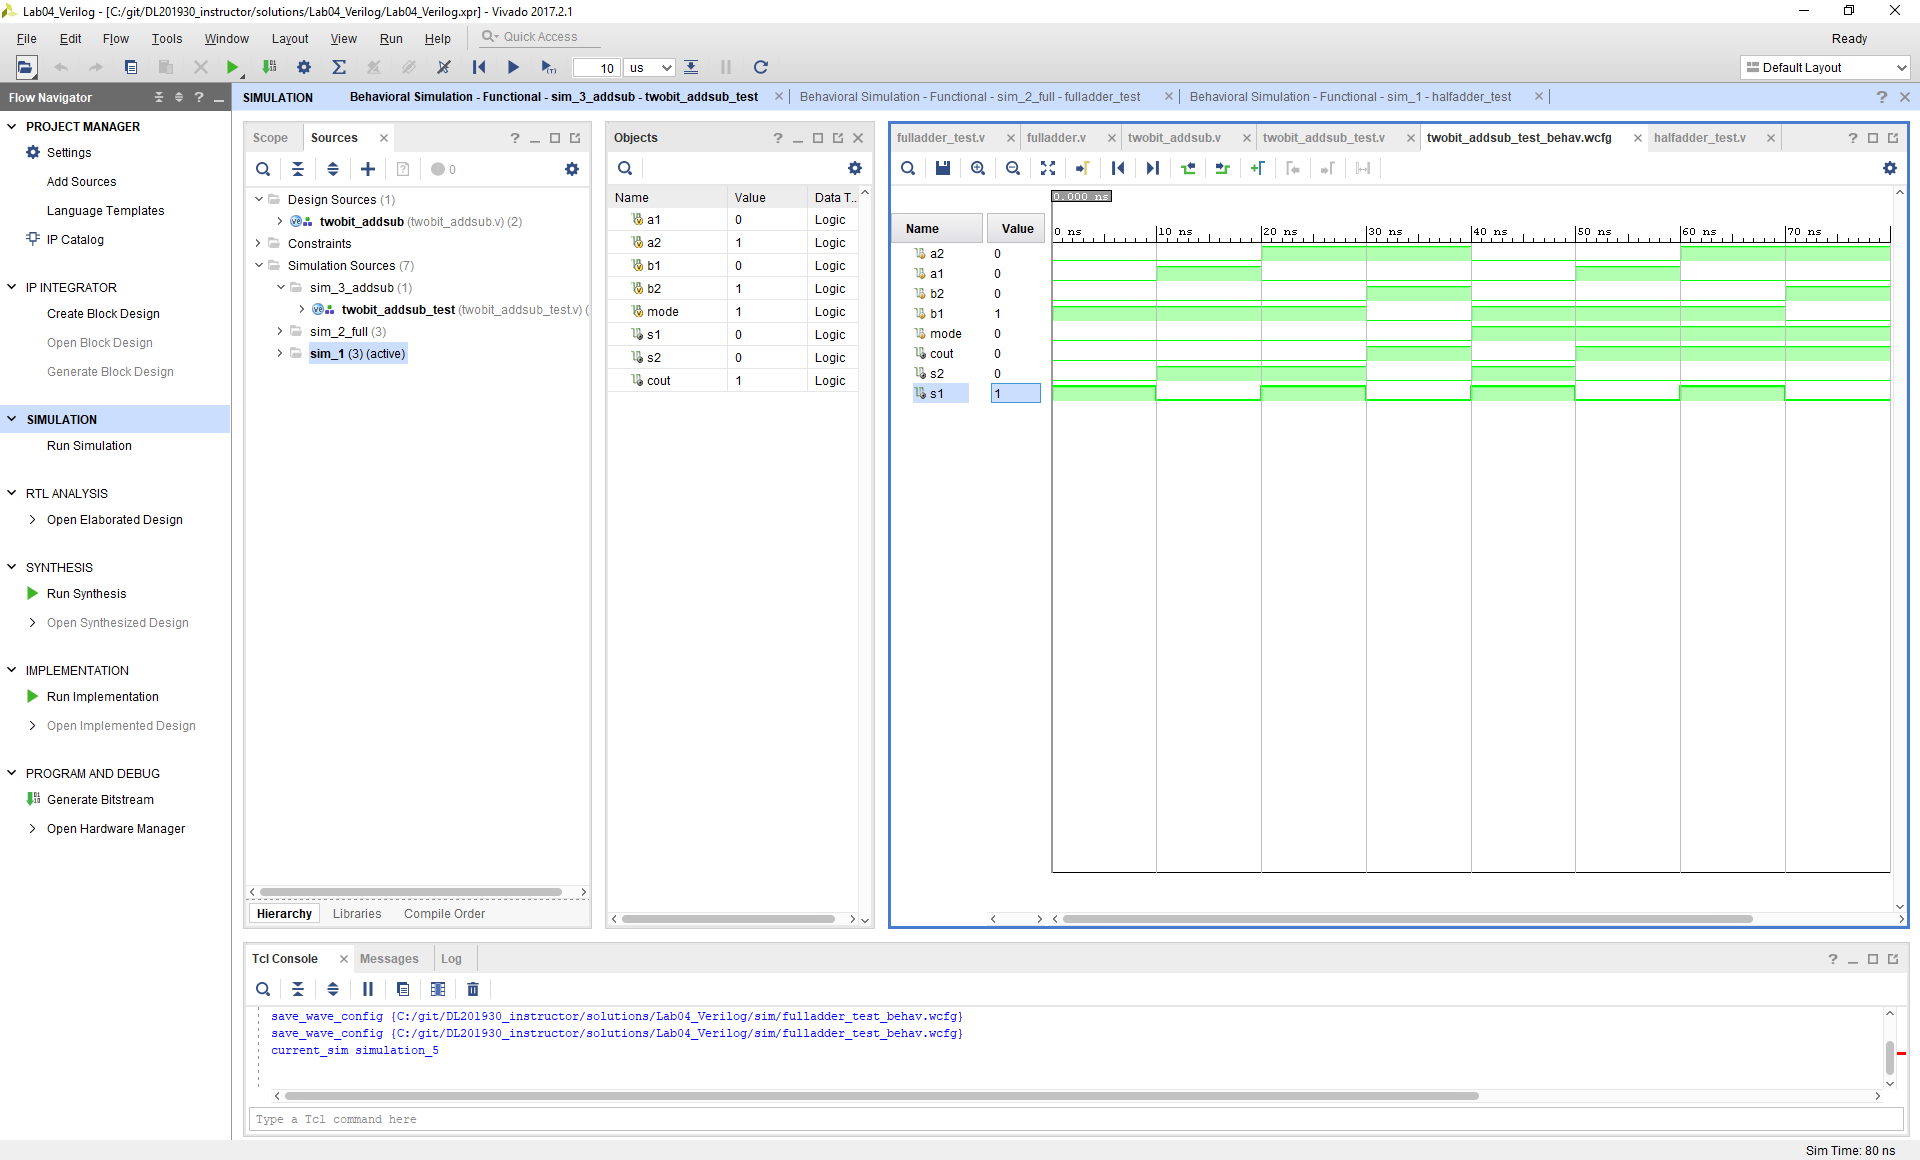
\includegraphics[width=\textwidth, trim=550 450 15 130, clip] {lab1_example_screenshot}
		\caption{Table and Simulation waveform to reproduce}
		\label{fig:sim_with_table}
	\end{figure} 
 
	\begin{figure}\centering
		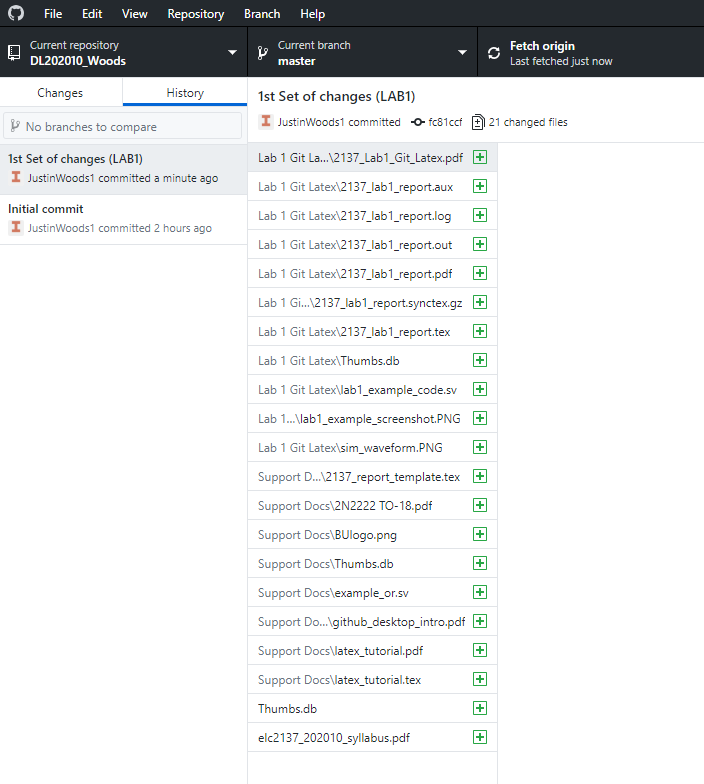
\includegraphics[width=\textwidth]{Capture}
		\caption{Screenshot of GitHub}
		\label{fig:sim_with_table}
	\end{figure}

\end{document}
